%%  ***************************************************************************
%% My paper
%%
%% Authors: Emmett Brown, Marty McFly, Biff Tannen
%%
%% NOTE: this file will not compile until you called the script
%% generate-preamble.php once. See the file Readme.md to understand what
%% to do.
%%
%% This paper is an instance of the PaperShell template. For more
%% information, please visit https://github.com/sylvainhalle/PaperShell
%%  ***************************************************************************
%% ---------------------------
%% Author preamble. Uncomment the one corresponding to the
%% stylesheet you want. **Don't forget to also uncomment the proper
%% line for the postamble at the end!!**
%% ---------------------------
%\input preamble-aaai.inc.tex
%\input preamble-acm.inc.tex
%\input preamble-acm-journal.inc.tex
%\input preamble-elsarticle.inc.tex
%\input preamble-ieee.inc.tex
%\input preamble-ieee-journal.inc.tex
\input preamble-lncs.inc.tex
%\input preamble-svjour.inc.tex

%% ---------------------------
%% If you wish to include additional packages, define new environments or
%% new commands, put them in the file includes.tex
%%
%% Write your abstract in the file abstract.tex.
%% ---------------------------

%% ---------------------------
%% Categories and keywords. Uncomment only for ACM.
%% See: http://www.acm.org/about/class/ccs98-html
%% ---------------------------
\begin{comment}
  \category{D.2.2}{Software Engineering}{Design Tools and Techniques}
  \category{D.2.4}{Software Engineering}{Software/Program Verification}
  \category{H.3.5}{In\-for\-ma\-tion Storage and Retrieval}{Online Information Services}[web-based services]
  \terms{Theory, verification}
  \keywords{Navigation, web applications, model checking}
  \vfill\eject
\end{comment}

%% ---------------------------
%% Introduction
%% ---------------------------
\section{Introduction} %% {{{

Fault localization. 

While lot of work has been done on reporting the presence of an error, much less has been done on localizing the fault, i.e.\ identifying artifacts providing a meaningful explanation for the occurrence of the fault.

%% }}} --- Section


%% ---------------------------
%% Introduction
%% ---------------------------
\section{Witnesses} %% {{{



%% }}} --- Section


%% ---------------------------
%% A section
%% ---------------------------
\section{Conclusion} %% {{{

It works.

\begin{figure}
  \centering
  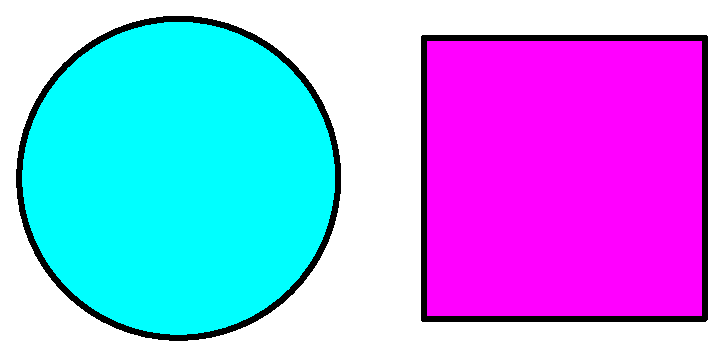
\includegraphics[width=0.4\textwidth]{fig/square-circle}
  \caption{A square and a circle}
  \label{fig:square-circle}
\end{figure} 

%% }}} --- Section

%% ---------------------------
%% Bibliography. Uncomment the one corresponding to the
%% stylesheet you want.
%% ---------------------------
%\input postamble-aaai.inc.tex
%\input postamble-acm.inc.tex
%\input postamble-acm-journal.inc.tex
%\input postamble-elsarticle.inc.tex
%\input postamble-ieee.inc.tex
%\input postamble-ieee-journal.inc.tex
\input postamble-lncs.inc.tex
%\input postamble-svjour.inc.tex

\end{document}

%% :folding=explicit:wrap=soft:mode=latex:
